\documentclass{article}

% if you need to pass options to natbib, use, e.g.:
% \PassOptionsToPackage{numbers, compress}{natbib}
% before loading nips_2016
%
% to avoid loading the natbib package, add option nonatbib:
% \usepackage[nonatbib]{nips_2016}

\usepackage[final]{nips_2016}

% to compile a camera-ready version, add the [final] option, e.g.:
% \usepackage[final]{nips_2016}

\usepackage[utf8]{inputenc} % allow utf-8 input
\usepackage[T1]{fontenc}    % use 8-bit T1 fonts
\usepackage{hyperref}       % hyperlinks
\usepackage{url}            % simple URL typesetting
\usepackage{booktabs}       % professional-quality tables
\usepackage{amsfonts}       % blackboard math symbols
\usepackage{nicefrac}       % compact symbols for 1/2, etc.
\usepackage{microtype}      % microtypography
\usepackage{xcolor, graphicx, subcaption, float, enumitem, amsmath}

\newcommand{\selfnote}[1]{\footnote{\textcolor{red}{#1}}}
\newcommand{\domainDoubt}[1]{\footnote{\textcolor{teal}{#1}}}
\newcommand{\technicalDoubt}[1]{\footnote{\textcolor{blue}{#1}}}

\title{Commuter classification and behavior clustering: Beijing use case}

% The \author macro works with any number of authors. There are two
% commands used to separate the names and addresses of multiple
% authors: \And and \AND.
%
% Using \And between authors leaves it to LaTeX to determine where to
% break the lines. Using \AND forces a line break at that point. So,
% if LaTeX puts 3 of 4 authors names on the first line, and the last
% on the second line, try using \AND instead of \And before the third
% author name.

\author{
  Selene Baez  Santamaria \\
  \texttt{s.baezsantamaria@student.vu.nl}
}

\begin{document}
% \nipsfinalcopy is no longer used

\maketitle

\begin{abstract}
  Public transportation, centered on subway and bus networks, is an data-rich domain that can benefit from data mining and machine learning techniques. The classification of commuters versus non-commuters/occasional travelers can help government, transport management and operators to better target their policies in order to improve the transportation network in large cities. Furthermore, characterizing commuters by behavior clustering can bring deeper insight into their needs and routines as a whole. 
  This project proposes the usage of ensemble models for classification and clustering of public transport users. For this purpose, transit card data will be used, available from the city of Beijing, China. 
\end{abstract}

\newpage

\tableofcontents

\newpage
\section{Introduction}

\subsection{Transportation domain}
Urban public transportation includes systems that are available for use by anyone in urban areas. Its facilities are commonly composed by buses, subway/metro lines, light rails, tramways, trains, taxis and others. As a network, they provide service for the majority of citizens in urban areas.\citep{vuchic1900urban}

Figure \ref{fig:transportation/passenger} shows the passsenger transport usage, as million passengers per kilometer. This represents the transport of a passenger for one kilometer. From the top image we note that United Stated, China, Germany, France, Italy, and United Kingdom contitute the six countries with the most passenger transport, according to their reported data from 2015 or later.\cite{OECD2017passenger} 

Furthermore, historical data in the bottom image reveals the 15 years behavior for each of the aforementioned countries. Most of the countries show stability, with increase or decrease of less than .10 million passengers for European countries, and .5 million passengers for United States. China, however, shows a trend with steep increase for most of the selected years. In fact, comparing to its less than 1.2 million passengers in 2000, China doubled its public transport usage to 2.4 million passengers in 2015. 

\begin{figure}[H]
  \centering
  \begin{subfigure}[b]{.85\textwidth}
  	\centering
  	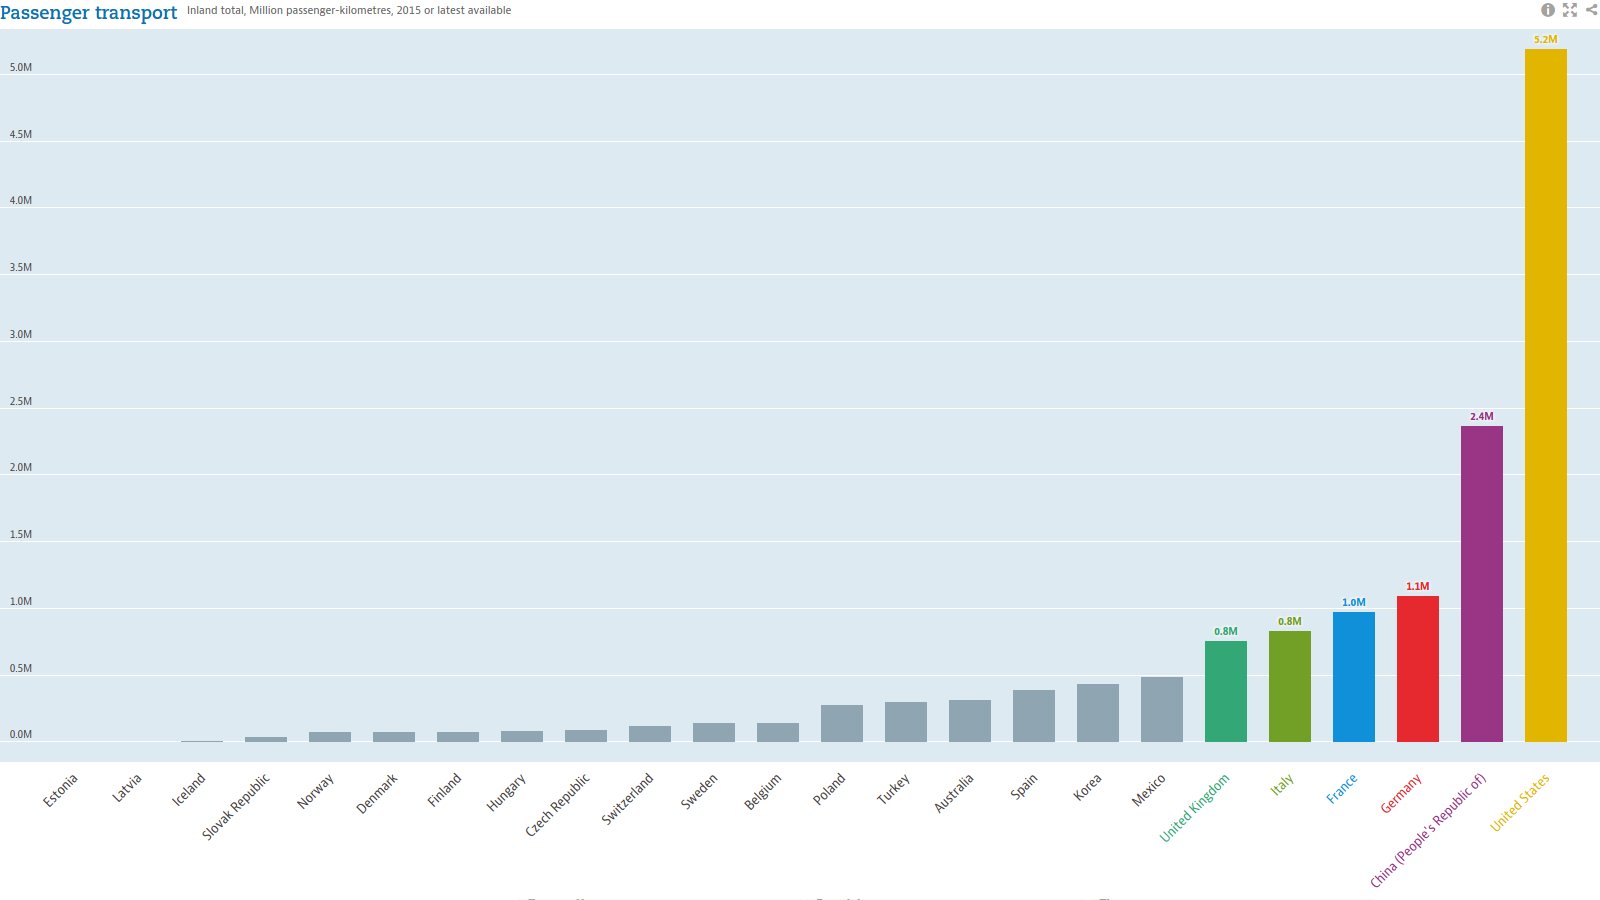
\includegraphics[width=\linewidth]{./images/OECD_passengers_absolute.png}
  	\caption{Passenger transport data, per country.}
  \end{subfigure}
  \begin{subfigure}[b]{.85\textwidth}
  	\centering
  	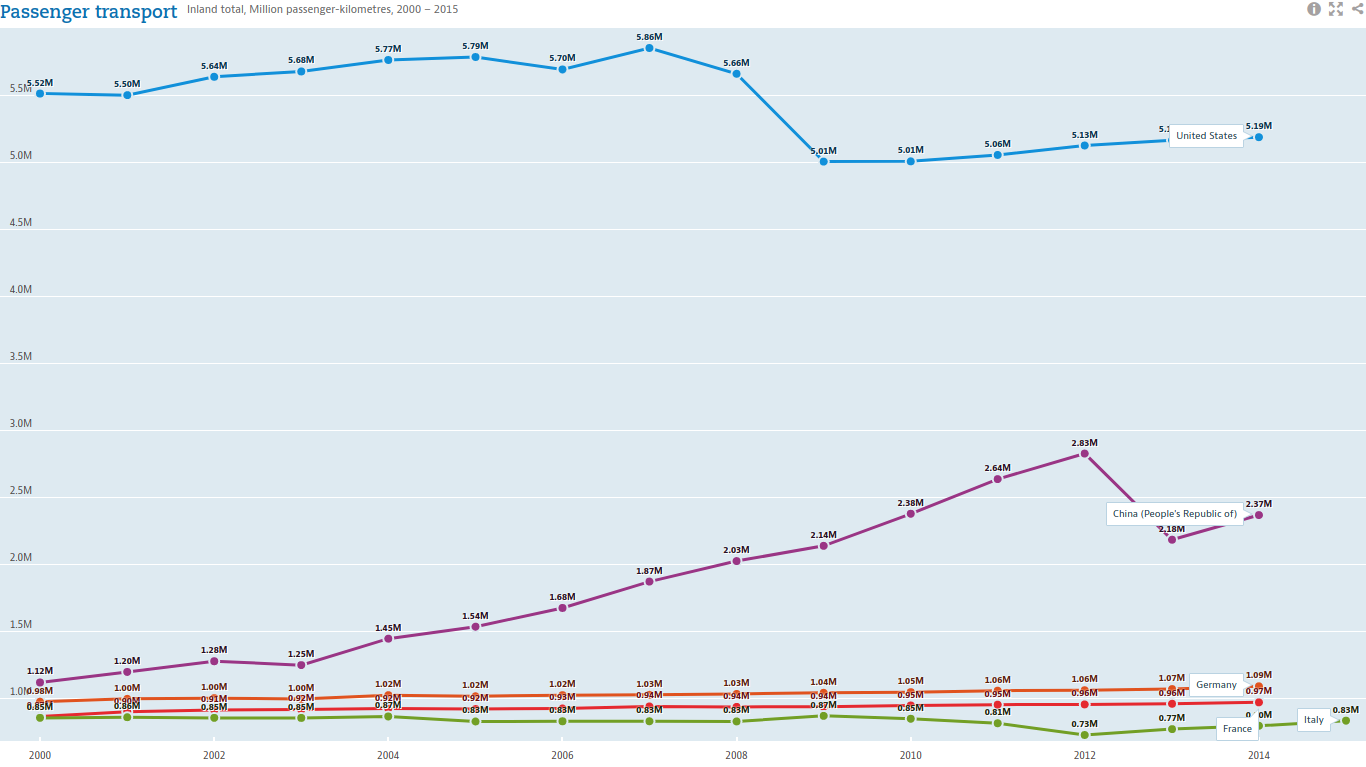
\includegraphics[width=\linewidth]{./images/OECD_passengers_increase.png}
  	\caption{Historical data for the top six countries with most passenger transport usage.}
  \end{subfigure}
  \caption{OECD countries and their passenger transportation data.}
  	\label{fig:transportation/passenger}
\end{figure}

Though it is a more sustainable alternative compared to private car usage, public transport usage has a significant environmental impact, affecting noise and air pollution. Diesel buses, which generally make up a major part of public buses, have large fuel consumption needs and contribute significantly to CO$_{2}$ emissions. Even eco-friendly alternatives such as hybrid diesel buses are sensitive to operating conditions, as their fuel consumption may increase by up tp 50\% when the on-board air conditioning is on.\cite{zhang2014real}

Consequently, public transportation directly relates to energetic demand, since its facilities are mostly petroleum or electrical based. In terms of global energy consumption, passenger transportation accounts for about 25\% of the total world energy consumption. Furthermore, the tarnsportation sector consupmtion increases at an annual average rate of 1.4.\% \cite{eia2016energy} This may bring further economical implications for countries with high public transportation demand.

\subsubsection{Who are the commuters?}
A major proportion of public transport users is represented by commuters. These are regular users of public transit, with consistent spatio-temporal patterns in their travels. Driven by a routine, commuters travel back and forth from specific places, commonly represented by their home, work, school, or other similar locations.

As commuters are frequent users of public transit, the  conditions of the public network directly influence their personal well being and generally impacts their quality of life. Intuitively, if the commuting experience is unpleasant, daily travel can bring distress to commuters and even repel them from using the public transport at all. Several studies have looked into public transit evaluation from different perspectives, including commuters' needs \cite{mao2016commuting}. The most common aspects of it include: travel time, average speed, delays, accessibility, service coverage, crowded level, facilities quality, and fare rate. Weng et al \cite{weng2013bus} identified five categories (Convenience, rapid, Reliability and Comfort) that summarize commuters priorities when choosing to travel by public transport.
 
From both of the above, the large presence of commuters and their known needs and preferences, it follows that identifying commuters can help in creating a sustainable public transportation network. Public transit stakeholders should be able to understand the commuters' demands and its dynamics, consequently bringing long term planning and policies for improving the overall commuting experience.

\subsection{The city of Beijing}
The city of Beijing presents a special case of urbanization and rapid industrialization. This is reflected in a sudden population growth of 20\% per decade since 1960, with the largest increase of 44\% in the last ten years. The latest official census in 2010 reported the urban agglomeration of Beijing (including Beijing itself and its adjacent suburban areas) having a population of 19,612,368 people. The UN World Urbanization Prospects estimates the 2017 population at over 22 million inhabitants. \cite{world2016beijing}

As a result of the population explosion, many environmental and social resources are under pressure. From the environmental side, one of the most notable issues is related to air pollution, due to the significantly high pollutant emissions in the city \cite{zhang2016air}. Similarly, the city's downstream river pollution is serious, with most regions of the Yellow river being unable to comply with the lowest water quality standards. \cite{wang2015studies} 

In the aspect of social resources, one of the main complications is the one of mobility. In Beijing, public transport is the dominant mode of transportation, accounted for 44.0\% of all trips compared to 32.6\% attributed to private cars \cite{mao2016commuting}. In 2008, the total ridership was 6.5 billion travels. Though it is continually expanding, it is a fact that public transport is overcrowded, constantly reaching over 100\% capacity \cite{beijing2009research}.

Beijing public transport is composed of buses, subway and bicycles. The three types can be accessed by using a single smart card. 

\begin{description}
\item[Bus:] In 2015, there were 876 bus lines with 23,287 buses in operation. The bus network is the most extensive mode of transportation, expanding over 20,186 km. It observes an average daily traffic volume of 10.98 million passengers, with the highest daily volume reaching 13.07 million on one day. \cite{beijing2016annual}

\item[Subway:] The Beijing subway has 18 lines with 334 stations, of which 53 are transfer stations. In 2015 it had an operating length of 554 km, with 5,024 vehicles running. \cite{beijing2016annual} Its network is is split by two operators: the state-owned Beijing Mass Transit Railway Operation Corp (operating 15 lines), and the joint Hong Kong venture Beijing MTR Corp (operating 3 lines).

Beijing's subway has an average daily traffic volume of 9.11 million passengers, with a maximum recorded volume of 11.66 million passengers. As such, it is the second busiest metro system in the world, providing 3,410 million annual journeys. Compared to the service provided in 2012, the system observed a 39\% increase in usage by 2014. It is also the second longest metro network, surpassed by Shanghai by only 21 km.  \cite{uitp2015world} 

\item[Bicycles:] Beijing first implemented public bicycle systems in 2012. As of 2015, in total, 67,000 bikes are available for rental with 2,700 pick up/drop off points spread across the city. \cite{beijing2016annual}
\end{description}

\subsection{Motivation}
This project performs an interdisciplinary study between the areas of Artificial Intelligence and Metropolitan Transportation. It is focused on introducing data mining techniques to a data rich domain. 

The area of Artificial Intelligence is able to provide dozens of prediction algorithms. Though constantly under refinement, it is time for state-of-the-art techniques to be applied to real and large impact situations to test their ability to deal with noisy streams. Comparably, given the ever growing complexity of urban mobility, domain experts must focus on analyzing trends and insights instead of curating and making sense out of raw data. Therefore, both areas benefit from this project.

\subsubsection{Societal context}
Looking at the social context of Beijing, there are several reasons justifying an in depth study of commuters. 

First, a survey conducted in 2009 showed that 80\% of the public transport passengers' complaints in Beijing were related to the network being slow and time-consuming, inconvenient to transfer, unpunctual and unreliable. Commuters use the public transport network regularly to perform their routines, and thus need efficient and reliable means of transportation. Flaws and failures in the network reduce the attraction of public transport. \cite{beijing2009research}

Second, the city of Beijing faces a large imbalance between residential and working areas. Due to urban expansion, most residents have been forced to move to suburban areas due to the lack of affordable housing \cite{zhou2014commuting}. Targeting this group brings the largest benefits to the public.  

Third, government, transport management and operators can gain invaluable spatial and temporal insights regarding commuters' behaviors. This insight can lead to tangible results, including policies for increasing the efficiency of the public transit network, adjustable travel fares tailored to most relevant commuters' patterns, incentives to relieve peak hours and thus traffic congestion, urban planning for residential and industrial land use, and others.

\subsubsection{Scientific context}
From a scientific point of view, mobility patterns in metropolitan areas follow swarm behaviors. Based on individual travels and routines, travelers exhibit distinguishable characteristics on a larger scale. Both levels of understanding are crucial for Transportation experts. 

Surveys are the most widely used research method in metropolitan transportation studies. They are targeted to reach travelers on an individual level, while aggregated measurements are taken to investigate their collective behavior. The analysis is usually based on statistical methodology. 

These methods have several disadvantages. On the one hand, surveys are costly to implement, and in general have problems related to small populations and non-representative samples. Even when the latter problems are escaped, the typical quality versus quantity trade off is present, reducing the confidence of the collected information. Furthermore, surveys are based on self-report, which by itself has bias problems. On the other hand, aggregated measurements miss the interactions between individuals that cause the collective behavior. 

\textbf{Big Data}
In the last years, smart card systems have become more popular, making it possible to monitor travelers transactions and facilitating fare collection. Several cities have implemented such systems, for example the Octopus card in Hong Kong\cite{chau2003octopus}, Oyster card in London \cite{blythe2004improving}, OV-chipkaart in The Netherlands \cite{de2008analysis}, and Yikatong card in Beijing \cite{chan2010tactical}, to name a few.

In Beijing, over 90\% of public transit users are smart card holders. There is a significant incentive for using the Yikatong smart card since bus rides are heavily subsidized (the user has only to pay 50\% of the full price)\cite{ma2017understanding}. Moreover, the Yikatong smart card system is also integrated with taxi, electricity and sewage payments. 

Clearly, technology for transit data collection is broadly spread around the world. Transit smart cards are capable of recording spatio-temporal information at an individual level over long periods of time. This generates a large volume of historical data that only big data techniques can deal with. Furthermore, machine learning and other mining methods specialize in analyzing disaggregated complex information. As such, bringing state-of-the-art techniques into the Metropolitan Transportation domain can aid to unravel massive human behaviors and reveal patterns and trends in mobility.

\subsection{Thesis organization}
This Thesis is organized as follows:

First we perform a literature review to look for previous work on mining smart card transit data and for specific state-of-the art methodologies for classification and clustering complex spatio-temporal data. Subsequently, we establish the scope and research objectives of this project. We continue to describe the methodology thoroughly, including the data and the approach to mine it. Following this description, we identify three distinct stages of the project (Commuters classification, Variables evaluation, and Commuters clustering) and report their corresponding experimentation. Next, we discuss the findings and gather conclusions. Finally, future work opportunities are explored. 


\newpage
\section{Literature review}
In this section we look at studies within the last decade that are related to smart card transit data, and the clustering techniques for their mining. 

\subsection{Data mining on transit card data}
With the introduction of smart card systems in large cities, several studies have aimed to extract knowledge from the large amounts of data collected. Though different in their methodology, results concerning commuters are duplicated across studies. The spatial and temporal regularity of their travel is evident in their smart card data.

%Preprocess data by Wang in BJUT lab. \cite{wang2014research}

Morency et al. study spatio-temporal variability in Canadian smart card data. On the one hand, they examine spatial variability by measuring the number of distinct stops a smart card user visits, and the frequency of each stop. On the other hand, they examine temporal variability by clustering the boarding times of each smart card. Using these features, they observe the week to week variability for each of the five types of transit card available (Adult-interzone, Adult-express, Adult-regular, Elderly and Student). Their findings show that commuter type of cards visit a smaller range of bus stops compared to non-commuter types. Therefore, a small number of stops account for a high proportion of commuter's boardings. Additionally, commuters have the highest proportion of zero-boarding days on weekends \cite{morency2007measuring}.

%Density Based Scanning Algorithm with Noise to classify travelers according to their travel patterns.  \cite{ma2013mining}

Bhaskar et al. are concerned with passenger segmentation using Australian smart card data. First, they perform a two level DBSCAN algorithm for investigating spatial patterns, where the first level clusters Destination stops and the second level clusters Origin stops.  From this they extract frequent Origin-Destination (O-D) pairs. Separately, they applied DBSCAN to temporal features to determine most frequent boarding times.  As such, they characterize each user by the percentage of journeys they perform between the regular O-D, and the percentage of journeys they perform during their habitual times. Users with at least 50\% spatial and temporal regularity are thus classified as transit commuters; while users with no evident spatial or temporal pattern are classified as irregular passengers. The authors find that while most (64\%) of the passengers riding the public transit are irregular passengers, it is transit commuters who bring the most (46\%) revenue. Furthermore, they find that irregular passengers prefer high frequency routes significantly more than transit commuters, arguing that commuters are usually on a time habit, and thus are more willing to check and adapt to public transit timetables. \cite{bhaskar2015passenger}

Machine learning for commuters identification. SVM with 94\% accuracy. \cite{tu2016impact}

Langlois et al. present an innovative representation for smart card data. Using four weeks worth of data from London Oyster cards, they represent the card information as a time-ordered sequence of inferred activities.  11 clusters are found and characterized by evaluating socio-demographic variables like age, employment, annual household income, children per household and vehicles per household. The authors further grouped the clusters under "working day", "home bound", "complex activity pattern" and "interrupted pattern" categories. Their findings show that four clusters, grouped under the "working day" category have significantly different activities during weekdays as compared to weekends, with some avoiding transit during the weekends and others visiting different areas.  Four more clusters, grouped under the "home bound" category, are characterized by staying mostly at their primary area and low number of traveled days. \cite{langlois2016inferring}

One of the latest work on the field corresponds to Ma et Al. The objective of their work is to determine a scoring function for travelers that can correctly identify them as commuters, or non-commuters. In their work, they cluster stops using an improved DBSCAN algorithm. They engineer features for representing the frequency in which travelers follow spatio-temporal patterns. Travelers are then clustered according to these features following the ISODATA algorithm. As an output of the clustering, optimal cutoff levels in the scoring function were determined. As a result, evaluating a traveler does not depend on clustering centroids, but only on calculating the commuting score. This, as expressed by the authors, reduces computing time and treats each traveler independently from the others, which is not true for clustering algorithms \cite{ma2017understanding}.

A common practice, as used by \cite{ma2017understanding}, \cite{langlois2016inferring}, and \cite{morency2007measuring} is to divide the day into -hourly or half-and-hour- time bins. Bhaskar et al. recognize this as a problem in the field, by pointing out that this segregates journeys from 9:59 AM and 10:01 AM even though they intuitively belong to the same behavior. 

\subsubsection{Volume of data}
The volume of data collected by smart card systems is massive and is usually impossible to analyze all of it at once. The volume of the samples analyzed by previous work ranges from hundreds of smart cards to tens of millions of smart cards, leading to up to hundreds of millions of individual smart card transactions. The details are summarized in Table \ref{table:volumeData}.
 
\begin{table}[H]
\centering
\begin{tabular}{||c c c c c||} 
 \hline
 Authors & Year of publication & Records & Unique smart cards & Time span \\ [0.5ex] 
 \hline\hline
 Tu et al. \cite{tu2016impact} & 2016 & Unknown & 978 & one week \\ 
 Morency et al. \cite{morency2007measuring} & 2007 & 2.2 million & 7,118 & 277 days \\
 Langlois et al. \cite{langlois2016inferring} & 2016 & 3 million & 33,026 & four weeks \\
 Bhaskar et al. \cite{bhaskar2015passenger} & 2015 & 34.8 million & 1 million & 4 months \\ %, working days only
 Ma et al. \cite{ma2013mining} & 2013 & Unknown & 3 million & one week \\
 Ortega \cite{ortega2013classification} & 2013 & 65 million & 5.7 million & one week \\
 Ma et e. \cite{ma2017understanding} & 2017 & 364 million & 18 million & one month\\ [1ex] 
 \hline
\end{tabular}
\caption{Volume of data analyzed by different authors}
\label{table:volumeData}
\end{table}


\subsection{Classifying and clustering spatio-temporal data}
Human mobility is intrinsically tied to spatio-temporal properties. Still, the greatest amount of studies analyze public transit journeys by separating spatial features from temporal features.


\subsubsection{Clustering algorithms} 

\textbf{Hierarchical clustering}

Langlois et al. use agglomerative hierarchical clustering for areas clustering. In order to infer the user-specific activities, all stops or stations visited by each user are clustered by merging the two closest areas until a threshold distance is reached. Their algorithm also considers the distance between stops and the frequency of travel between them. Therefore, different activities are likely to be associated with different areas \cite{langlois2016inferring}.

\textbf{Partitional clustering}

K-means algorithm is the most widely used method for partitional clustering. It requires having a predefined number of clusters to fit the data to. 

Morency et al. use K-means for clustering hourly boarding times according to card type. They apply Hamming distance (representing the percentage of data between two elements) and a combination of batch and online updates. Through empirical tuning, they select to find four clusters per card type. It is worth noting that by using a card-day unit, they allow a card to belong to a different cluster according to the day of travel. As every card type is composed of four boarding patterns, travelers are not restricted to follow a routine everyday, but can exhibit different behaviors on different days. For example, the Adult-regular card type contains a 9:00AM-and-5:00PM-boarding cluster and a no-boarding cluster. Thus, a user of this card could belong to the first cluster on weekdays and to the second cluster on weekends.  \cite{morency2007measuring}

Bhaskar et al. apply K-means for binary classification purposes. As such, they classify frequent and infrequent transit users, using the number of traveled days and the number of journeys made as features. Unfortunately, K-means performs poorly since no distinct clusters are evident. The most likely cause for the previous is the strong correlation between traveled days and journeys, combined with the authors oversight of whitening and standardization techniques. \cite{bhaskar2015passenger}

Langlois et al. use K-means to find clusters of activity sequences. They employ specialized sampling techniques, like bootstrapping, to deal with big data.  Moreover, they tune the algorithm parameters using the DB-index, which is the ratio of the within cluster distances to the across cluster distances. They find two optimal number of clusters (4 and 11), out of which they select the largest to provide the most detailed segmentation. They further perfection the algorithm by using k-means++initialization over 150 replications. Additionally, this paper acknowledges that clustering techniques are sampled based, which means different samples may find different optimal solutions. The authors validate their approach by analyzing the stability of the clusters over samples obtained at different points in time. By extracting the same number of clusters and fitting the samples to each set, they find that 91\% of users are assigned to their equivalent clusters. \cite{langlois2016inferring}

%k-nearest neighbor \cite{ortega2013classification}

\textbf{Density based clustering}

Density based algorithms excel at dealing with anomalies, since they ignore low density areas and interpret them as noise. They do not required a redefined number of clusters and adapt to find clusters of any size. The required parameters for DBSCAN are a maximum reach distance $\epsilon$ and the minimum number of points per cluster.

Bhaskar et al. use three DBSCAN algorithms to cluster Origin stops, Destination stops, and boarding times. For each of the previous, they tune the algorithm parameters by fixing a domain reasonable $\epsilon$ (1000 m walking distance or 5 min variance in boarding time), and selecting the minimum points by comparing the percentage of data considered to belong to any cluster as opposed to data considered to be noise given the par-specific parameters \cite{bhaskar2015passenger}. 

Ma et al. use an improved DBSCAN algorithm to cluster bus/subway stops. In their approach, abnormal stops are not considered noise, but are allowed to be re-clustered by splitting large clusters into several smaller clusters. 

Though clustering algorithms are common in the field, they are not always used for classifying users. For example, Bhaskar et al. use density based clustering for engineering regularity features. However, the classification of users is rule-based according to which feature (spatial or temporal regularity) is stronger in each user \cite{bhaskar2015passenger}. Morency et al. use partitioning clustering to characterize existing user categories according to their boarding times \cite{morency2007measuring}. 

\subsubsection{Features}
In general, scalar aggregated features are used for users characterization. Some examples are:

\begin{itemize}
\item \textbf{Frequency indicators:} number of traveled days \cite{bhaskar2015passenger} \cite{langlois2016inferring} \cite{ma2017understanding}, number of journeys \cite{bhaskar2015passenger}, number of times a stop was visited \cite{morency2007measuring}, number of days with zero boardings \cite{morency2007measuring}, most frequent home/work stop \cite{ma2017understanding}, most frequent home/work route \cite{ma2017understanding}, most frequent departure time from home/work \cite{ma2017understanding}, number of trips to the most frequent home/work stop\cite{ma2017understanding}, number of trips following the most frequent home/work route \cite{ma2017understanding}, number of trips during most frequent departure time from home/work \cite{ma2017understanding}

\item \textbf{Range/coverage indicators:} distinct stops visited \cite{morency2007measuring}, spread of days between the first and last journey \cite{langlois2016inferring}

\item \textbf{Calendar-based indicators:} observed day \cite{morency2007measuring}, day of week \cite{morency2007measuring}

\end{itemize}


Different from all others, Langlois et al. follow a unique methodology for engineering features. First, they represent the travel data per user using a three dimensional matrix where $x$ represents the day in the four week period, $y$ represents the hourly time bin, and $z$ represents the area where the inferred activity took place, encoded as a one hot vector. The authors perform Principal Component Analysis (PCA) for dimensionality reduction, based on Eagle and Pentland's eigenbehaviours \cite{eagle2009eigenbehaviors}. An analysis of the average correlation of the first 13 components, results in the selection of the first 8 components as the most informative and stable. The projections of a user sequence onto these components (called weights) constitute the features to be clustered using k-means. \cite{langlois2016inferring}





As a conclusion, we note that while there has been research applying basic clustering and classification algorithms, most studies lack further specialized data mining techniques for preprocessing data, tuning algorithms parameters, and/or visualizing results. 

\newpage
\section{Research objective}
The objective of this project is to identify and characterize commuters in the city of Beijing by using smart card data. As such, the underlying goal is to find patterns in the spatio-temporal data of public transport travelers, and interpret the results using domain knowledge by experts in the Transportation domain.  

\subsection{Research questions}
The min objective is further broken down into answering the following research questions: 

\begin{enumerate}
\item How accurately can commuters and non-commuters be identified using an ensemble model? How does this compare to the previous SVM model?
\item What is the minimal set of information needed from smart card data to reach an acceptable accuracy in classification?
\item To what extent is clustering commuters by its behavior informative to transportation specialists? 
\end{enumerate}

\subsubsection{Definition of terms}
A commuter is a public transit user whose smart card data reveals repeatable patterns in time and space. Though commuters are usually associated with Monday to Friday 9:00am to 5:00pm schedules, in this work we extend the definition to any routine travel pattern. 

A trip is a sequence of smart card transactions, including transfers, with an origin and destination. A trip is also represented as a record in the data, as it will be further explained in Section \ref{sec:data}

A transfer is a change in transportation mode. Transportation modes include Bus, Subway, and Bike. 

We make the assumption that smart card IDs and users have a one to one relationship, meaning each user has exactly one card and each card is used by exactly one user. As discussed with domain expert Quian Tu, although some people may own more than one card, this is a minority. Thus, the assumption holds for the majority of travelers. 

\subsection{Scope and structure}
This project is divided three main stages: 

\begin{description}[align=right,labelwidth=2cm]
\item[PART I] Classify commuters versus non-commuters by using an ensemble model. We examine the performance of our model and make a comparison with Tu's SVM model \cite{tu2016impact}. This is explored in Section \ref{sec:partI}.

\item[PART II] Revise features used in previous model in order to identify the most informative features and disregard redundant information. An extensive analysis of spatio-temporal properties will be done, combining transportation domain knowledge and statistical tools. This is explored in Section \ref{sec:partII}

\item[PART III] Commuters will be further clustered according to patterns in their travel behaviors. The clusters will be analyzed and interpreted to find distinctive characteristics that may be deemed as informative for transportation specialists. This is explored in Section \ref{sec:partIII}
\end{description}


\newpage
\section{Methodology}
\subsection{The data}
\label{sec:data}
Every record int the data represents a trip performed by a specific smart card. As such, it contains the following data fields:

\begin{itemize}
\item Data date: Year, month and day that the trip was made
\item Card code: Card identification number
\item Path link: Mode of transportation. B stands for bus, R for subway, Y for bicycle. Transfers between modes are shown by a dash. \footnote{Example: B-B represents a Bus to Bus transfer.} 
\item Travel time: Time spent in vehicles, measured in milliseconds
\item Travel distance: Distance traveled, measured in meters as performed by route. 
\item Transfer number: Number of changes in travel mode during the trip. 
\item Transfer total time: Total time spent in transfer, measured in milliseconds\item Transfer average time: Time spent in transfer, divided by number of transfers. Measured in milliseconds
\item Start/End time: Time stamp of when the trip started/ended. Date and time up to milliseconds precision
%Traffic zones
\item On/Off small traffic area: Integer ranging from 1 to 1911
\item On/Off middle traffic area: Integer ranging from 1 to 389
\item On/Off big traffic area: Integer ranging from 1 to 60
%Municipal zones
\item On/Off ring road: Integer ranging from 1 to 6
\item On/Off area: Integer ranging from 1 to 18
\item ID: record identification number created by joining the following: hour of the beginning of the trip | time stamp of beginning of the trip | card code performing the trip
\item Transfer detail: Mode of transportation, as well as line/route number and stations for boarding and alighting. More detail provided in Section \ref{sec:tripParsing}
\end{itemize}

Full privacy of card users is ensured, as there is no personal data linking card codes to specific individuals. 

The traffic zones (small, middle and big areas) are divided by the Beijing Municipal Institute of City Planning and Design (BICP). They are specific in different degrees, as shown in Figure \ref{fig:data/traffic_zones}. In general, the division principles correspond to the geopolitical environment and administrative planning, for example roads, villages and others. The 6 ring road and 18 areas districts are divided by the Beijing Municipal Government. The division is unique in Beijing. The 18 districts and counties are shown in Figure \ref{fig:data/18areas}. According to domain expert PhD. Liang Quan, these divisions are sufficiently informative for traffic analysis \cite{liang}.

\begin{figure}[H]
  \centering
  \begin{subfigure}[b]{.3\textwidth}
  	\centering
  	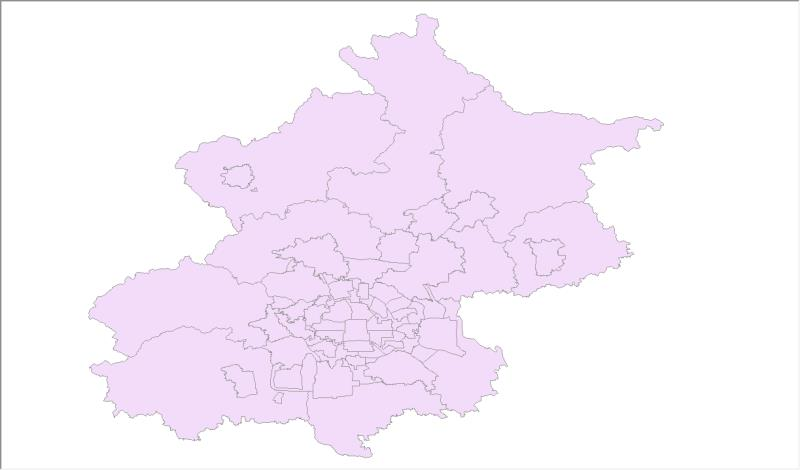
\includegraphics[width=\linewidth]{./images/big_traffic_zone.jpg}
  	\caption{Big zones}
  \end{subfigure}
  \begin{subfigure}[b]{.3\textwidth}
  	\centering
  	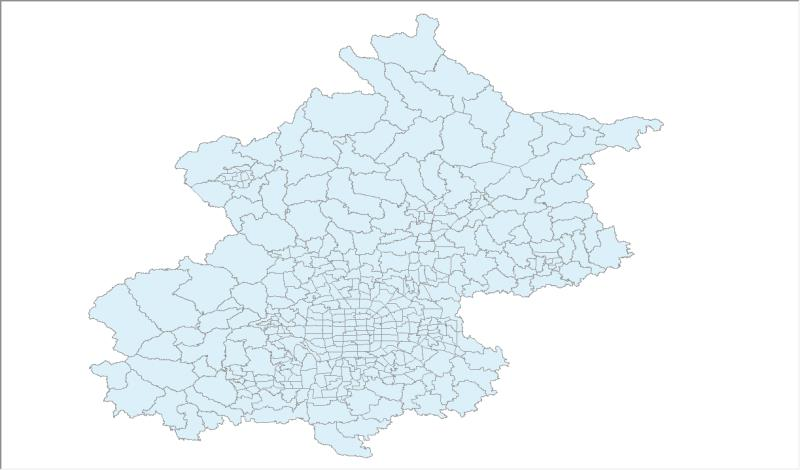
\includegraphics[width=\linewidth]{./images/middle_traffic_zone.jpg}
  	\caption{Middle zones}
  \end{subfigure}
  \begin{subfigure}[b]{.3\textwidth}
  	\centering
  	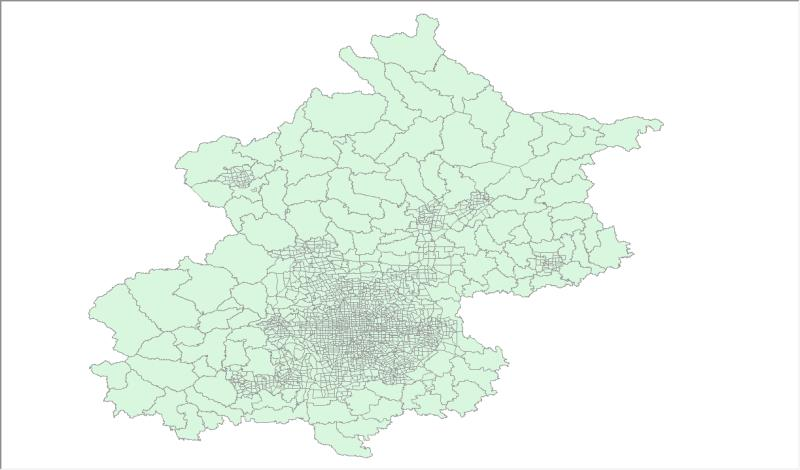
\includegraphics[width=\linewidth]{./images/small_traffic_zone.jpg}
  	\caption{Small zones}
  \end{subfigure}
  \caption{Traffic zone division}
  	\label{fig:data/traffic_zones}
\end{figure}

\begin{figure}
  \centering
  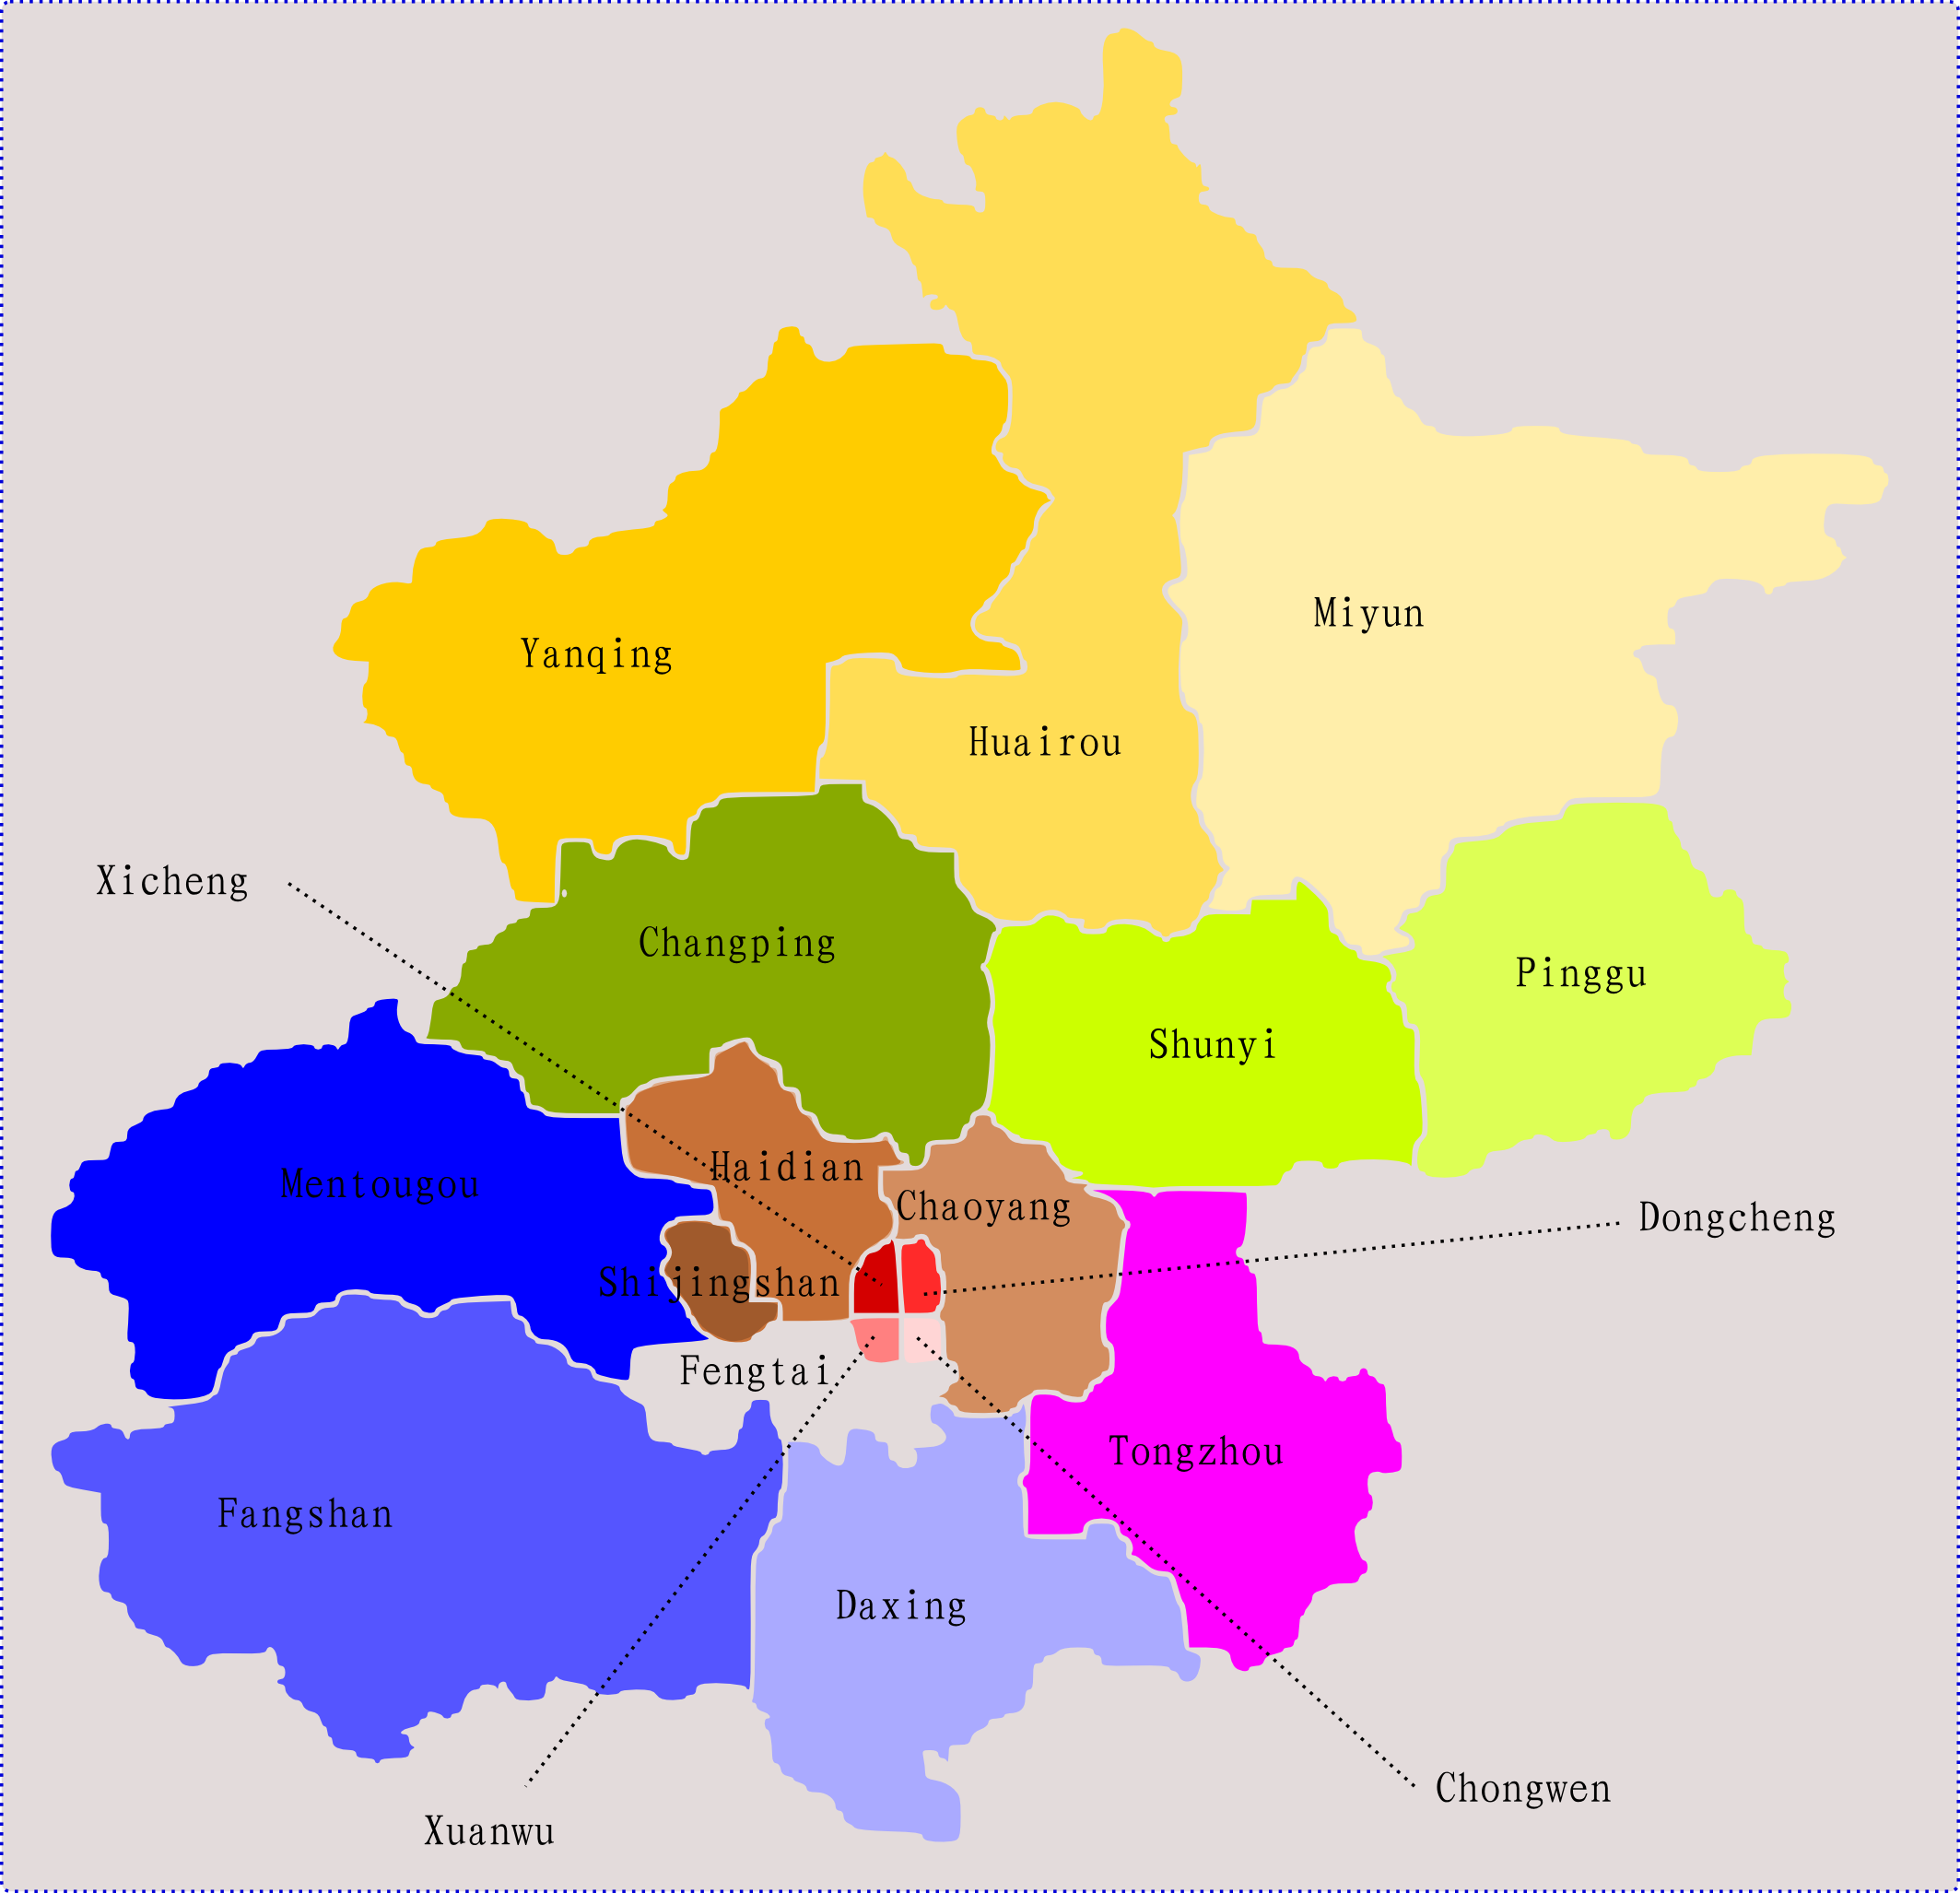
\includegraphics[width=.8\linewidth]{./images/beijing_18areas.png}
  \caption{Beijing's Districts and its Counties}
  \label{fig:data/18areas}
\end{figure}

Every day, more than 13 million records are collected, with approximately 5 million corresponding to subway trips, 8 million corresponding to bus trips and 100,000 corresponding to bicycle trips.

\subsubsection{Special considerations}
The previous description corresponds to the data as delivered by the Beijing Transportation Research Centre. As such, it has undergone some processing from the raw collecting phase. Some special considerations are explained below:


\begin{description}%[align=right,labelwidth=2cm]
\item[Travel distance by bike:] Since bicycles do not have predefined routes, the distance cannot be directly recorded. However, it is inferred by using the travel time and a static average speed for cyclist. 

\item[Subway transfer:] Transfers between subways lines cannot be tracked since a single check-in gives access to the traveler to all the subway network. In order to infer the transfer detail, the A* algorithm is used to calculate the most likely transfer sequence, given the boarding and alighting stations. 
Similarly to the bicycle missing information, the transfer time cannot be directly recorded. Using a static average walking speed and the known distance in transfer stations, the transfer time is calculated. 

\item[Transfer information:] The path link and transfer number fields are extracted from the transfer detail field. Similarly, the transfer average time is calculated from the transfer total time and transfer number fields. 
\end{description}


\subsubsection{Labeled and unlabeled data}
\begin{description}%[align=right,labelwidth=2cm]
\item[Commuter classification:]
Classification is a supervised learning task, where every training data sample requires an associated label determining its true class. In case of commuter classification, this translates to having smart card codes associated with either a "commuter" or "non-commuter" label. Such data is expensive and limited since it can only be obtained by asking the users directly if they are commuters or not. Thus, in general, annotated data is not available, and labeling new records falls beyond the scope of this project. 

As a solution for the above, we take advantage of the dataset used by Tu\cite{tu2016impact}. This dataset corresponds to trip records performed during a week in January 2015, and it contains labels for 978 smart cards, collected and validated via surveys. The original dataset distribution is composed by:

\begin{itemize}
\item 6439 records of 481 commuters
\item 1628 records of 497 non-commuters
\end{itemize}

For this project, the Beijing Transportation Research Centre has provided us with one month worth of data, corresponding to January 2015. In order to construct an extended labeled dataset, we take these 978 labeled smart card IDs and search for their corresponding records in the one month sample. This dataset is used for Part I (Section \ref{sec:partI}) and Part II (Section \ref{sec:partII}) of this project. 

\item[Commuter clustering:]
For this project, 100, 000 records are sampled every day for a month. In this case, the samples correspond to November 2014, which does not overlap with holidays and has a relatively stable weather thus diminishing the variance between bicycle and bus/subway traveler preferences.

\end{description}

\subsection{Data preprocessing}

\subsubsection{Cleaning}
As first step for preprocessing the data, we perform a cleaning where we eliminate records that are faulty, for example: 

\begin{enumerate}
\item Eliminate records with missing data: ~10.93\% records eliminated
\item Eliminate records with missing travel details: ~1.58\% records eliminated
\item Eliminate records with travel time <= 0: <0.01\% records eliminated
\item Eliminate records with travel distance <= 0: ~9.82\% records eliminated
\item Eliminate records linked to users with insufficient trips: ~ 25.89\% records eliminated when requiring at least 2 trips.
\end{enumerate}

This leaves ~51.76\% records available for usage. 

Insufficient trips regulated by a user input \selfnote{plot percentage of records and min records needed. Tune parameter}

\subsubsection{Trip parsing} 
\label{sec:tripParsing}
We parse the trip details using a combination of two techniques: regular expressions and tokenization. 

\textbf{Regular expression}
Since a trip may include transfers, we define a trip to be composed of one or many "rides"

In order to obtain the elements of each ride we look at the patters per travel mode.

    \begin{align*}
    BIKE &= (bike.STATION-STATION) \\
    SUBWAY &= (subway.LINE:STATION-LINE:STATION) \\
    BUS &= (bus.ROUTE(DIRECTION-DIRECTION):STATION \\
    &-ROUTE(DIRECTION-DIRECTION):STATION) \\ \\
    RIDE &= (MODE.[LINE/ROUTE:]?STATION-[LINE/ROUTE:]?STATION) \\
    TRIP &= RIDE [-> RIDE]? 
	\end{align*}    

\selfnote{change parenthesis to [(] or explain that they refer to literal parenthesis and not groups in regex}	
	
Subway lines and bus routes have number and letters as description. 

For bus routes, night, express and special routes are follow different paths, even if they are described with the same number. However, the direction in which they go is stable. 

For this reason we create a vocabulary with all unique parsed routes (without their directions)

\textbf{Tokenization}
Mode dictionary \selfnote{encode chinese in latex}



Example in Chinese -> English -> clean trip



\subsubsection{Data patching}
We note that the number of transfers and the path link are faulty. According to domain expert PhD. Tu Qiang, this must be recalculated \cite{tommy}. Figure \ref{fig:preprocessing/num_transfers} shows the distribution of the number of transfers per trip before and after patching.

\begin{figure}[H]
  \centering
  \begin{subfigure}[b]{.45\textwidth}
  	\centering
  	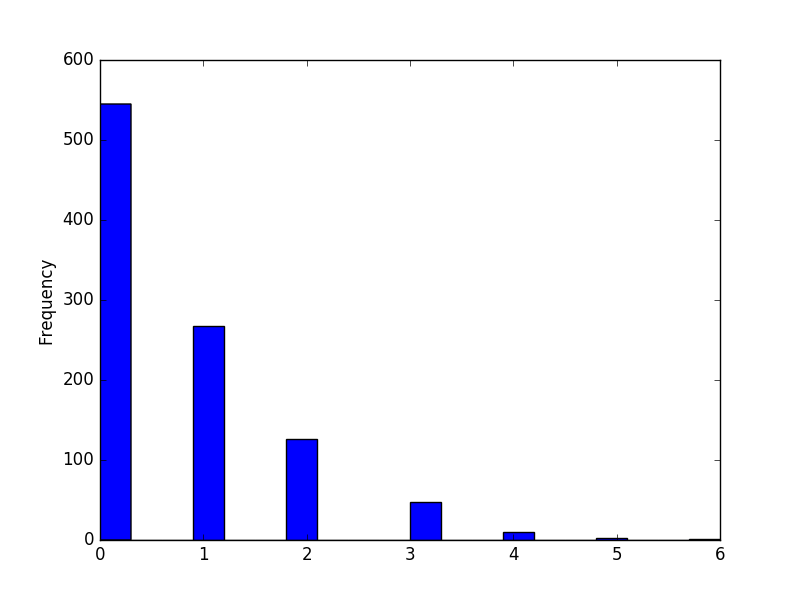
\includegraphics[width=\linewidth]{./images/num_transfers_hist.png}
  	\caption{Original}
  \end{subfigure}
  \begin{subfigure}[b]{.45\textwidth}
  	\centering
  	\includegraphics[width=\linewidth]{./images/num_transfers_recalculated_hist.png}
  	\caption{Recalculated}
  \end{subfigure}
  \caption{Transfer number distribution before and after recalculation.}
  	\label{fig:preprocessing/num_transfers}
\end{figure}

We note than most trips are performed without transfers, which is consistent with other studies \cite{bhaskar2015passenger}.

\subsubsection{Transformation and Standardization} \selfnote{replace images once run with all data}
Whitening vs standardization: whitening eliminates correlations between the data. In our case those are relevant and we ant to keep them. \technicalDoubt{Correlation between time and distance to be preserved?}Figure \ref{fig:preprocessing/distance_time_correlation} shows a clear correlation between travel distance and travel time. 

\begin{figure}[H]
  \centering
  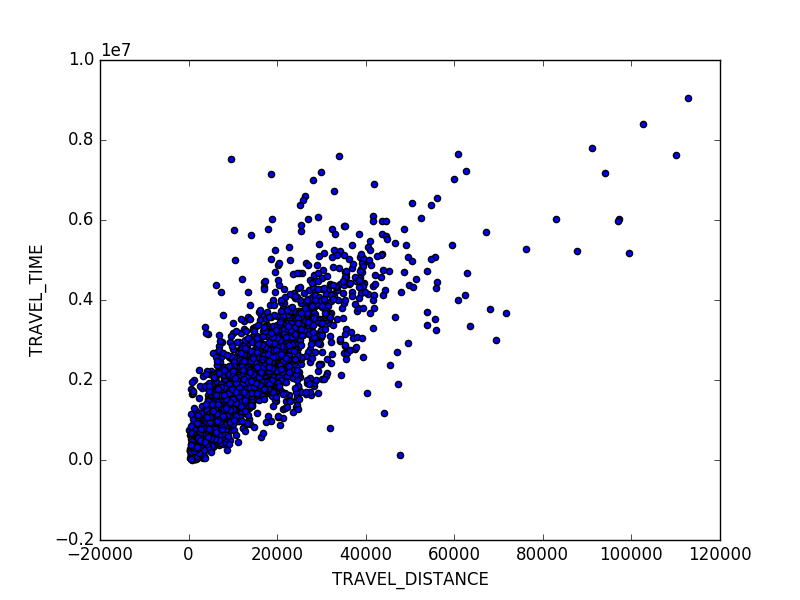
\includegraphics[width=.8\linewidth]{./images/distance_vs_time.png}
  \caption{Travel distance vs travel time.1000 record sample.}
  \label{fig:preprocessing/distance_time_correlation}
\end{figure}

Travel time and distance where standardized by subtracting the mean and forcing a unit standard deviation. As a result we observe a truncated Gaussian distribution $\mathcal{N}(\mu = 1, \sigma^2 = 1)$.

\begin{figure}[H]
  \centering
  \begin{subfigure}[b]{.45\textwidth}
  	\centering
  	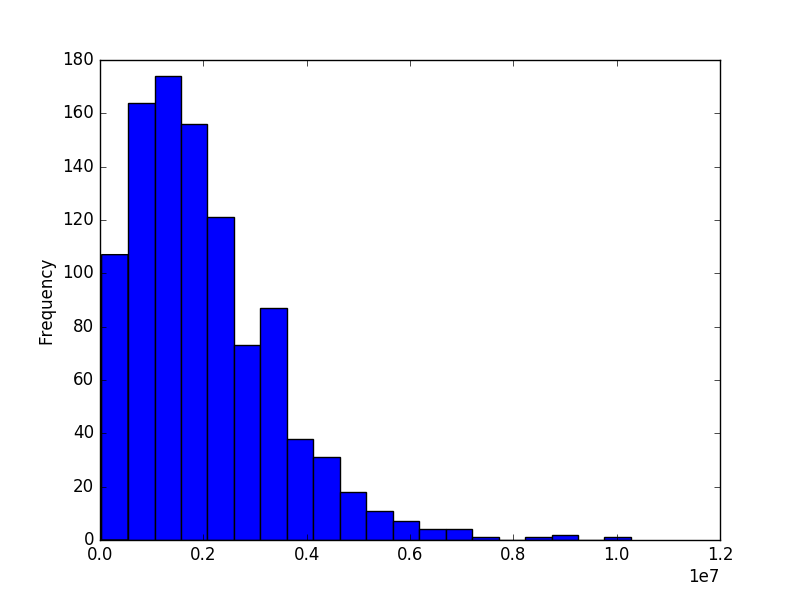
\includegraphics[width=\linewidth]{./images/time_hist.png}
  	\caption{Original}
  \end{subfigure}
  \begin{subfigure}[b]{.45\textwidth}
  	\centering
  	\includegraphics[width=\linewidth]{./images/time_standardized_hist.png}
  	\caption{Standarized}
  \end{subfigure}
  \caption{Time distribution before and after preprocessing. 1000 records sample.}
  	\label{fig:preprocessing/time}
\end{figure}

\begin{figure}[H]
  \centering
  \begin{subfigure}[b]{.45\textwidth}
  	\centering
  	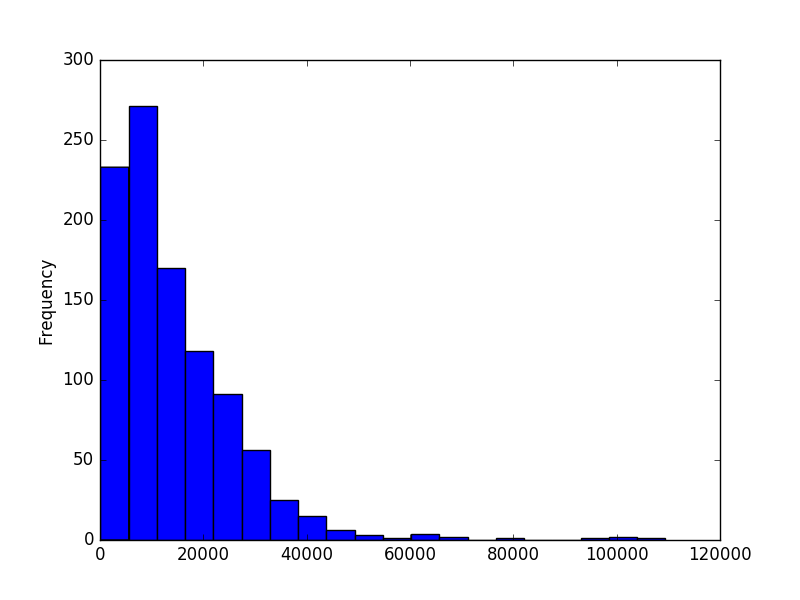
\includegraphics[width=\linewidth]{./images/distance_hist.png}
  	\caption{Original}
  \end{subfigure}
  \begin{subfigure}[b]{.45\textwidth}
  	\centering
  	\includegraphics[width=\linewidth]{./images/distance_standardized_hist.png}
  	\caption{Standarized}
  \end{subfigure}
  \caption{Distance distribution before and after preprocessing. 1000 records sample.}
  	\label{fig:preprocessing/distance}
\end{figure}
 

Regardless of its drawbacks, using hourly time bins is standard practice in the field \cite{langlois2016inferring} \cite{ma2017understanding} \cite{morency2007measuring}. From Figure \ref{fig:preprocessing/start_end_hour}, we note that our data follows the expected distribution for the domain, showing clear morning and evening peaks. 

\begin{figure}[H]
  \centering
  \begin{subfigure}[b]{.45\textwidth}
  	\centering
  	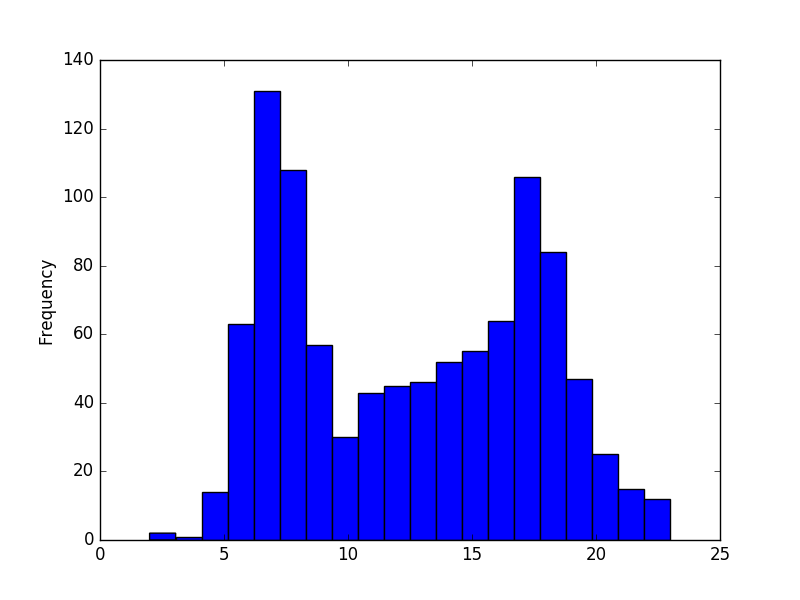
\includegraphics[width=\linewidth]{./images/start_hour_hist.png}
  	\caption{Start hour}
  \end{subfigure}
  \begin{subfigure}[b]{.45\textwidth}
  	\centering
  	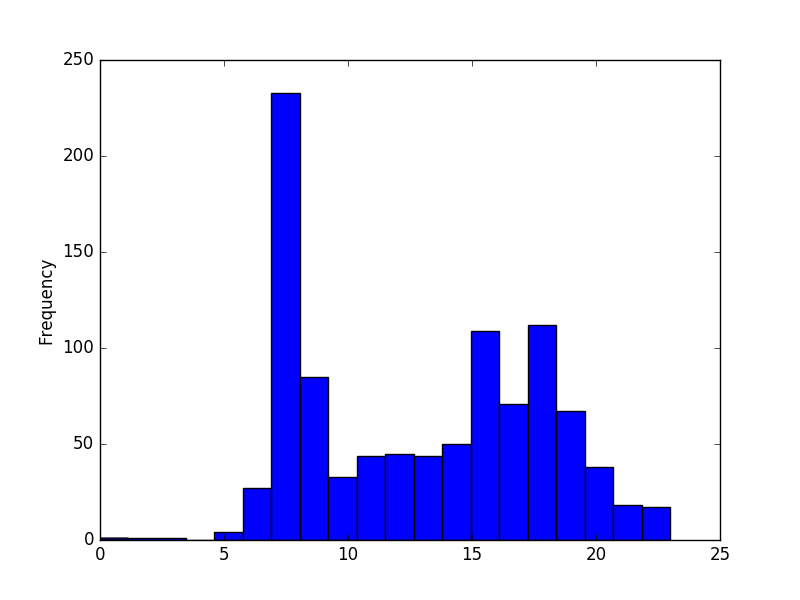
\includegraphics[width=\linewidth]{./images/end_hour_hist.png}
  	\caption{End hour}
  \end{subfigure}
  \caption{Distribution of start/end hours for trips.1000 records sample.}
  	\label{fig:preprocessing/start_end_hour}
\end{figure}


\subsection{Data mining techniques}
The work for this project is coded in Python, using libraries for data and numerical manipulation (\textit{Pandas}, \textit{numpy}), regular expressions (\textit{re}), machine learning (\textit{sklearn}), neural networks(\textit{Theano}).

\subsubsection{Spatio-temporal data structure}
The temporal factors to be explored are represented by the start/end times, as well travel/transfer time.

The spatial factors to be explored are represented by On/Off areas, lines/routes and stations. 

\begin{figure}[H]
  \centering
  \includegraphics[width=.9\linewidth]{./images/3D_structure.png}
  \caption{Spatio-temporal data structure.}
  \label{fig:preprocessing/3D_structure}
\end{figure}

Each plane corresponds to a feature. The x-y composition constructs a temporal structure between days and hours of the day. The advantage of this structure is its local properties, similar to image processing. Here, a temporal pixel is influenced by what happened in the previous/following hour (y axis), and on the previous/following day at the same time (x axis).

\selfnote{define temporal pixel as unit}
Each pixel may contain a trip feature vectors, which expands several layers.

Each layer is a feature, boarding spatial are in green, alighting spatial are in red, and other types of features are in yellow. 

Every user is represented as this structure. It is sparse, in that only a few time pixels are populated with trips, considering even regular public transport users do not perform more than 4 trips a day. 


\subsubsection{Feature engineering}
Considering around 15 features, we have $24 * 30 * 15 = 10,800$ pixels per user. Given the high dimensionality and the sparsity of the structure, we will perform dimensionality reduction. 

Taking advantage of the local properties of the proposed structure, we can apply convolutional filters to reduce the dimensionality to a more manageable number. 

The end result will be used as features for clustering commuters. 

\technicalDoubt{CNN chosen because of local properties, is PCA also local?}

\subsubsection{Ensemble models}
Ensemble models benefit from combining non-correlated methods. Classifiers might correct each other in specific hard cases. Ensemble models are chosen because of its robustness and modularity. Starting from a few simple classifiers, assembled via simple aggregation methods, the model can grow larger or more complex as needed.

\textbf{Supervised learning}
Decision trees, Bayesian classifiers and SVM are poweful enough. Bagging will be used to ensemble their predictions.

\textbf{Unsupervised learning}
The equivalent to ensemble models in unsupervised learning is consensus clustering.


\subsection{Correlation analysis}
chi-test


\newpage
\section{Commuters identification}
\label{sec:partI}
\subsection{Hypothesis}
As suggested by Tu \cite{tu2016impact} results, the data is almost linearly separable thus simple classifiers such as decision trees may suffice. 


\subsection{Model}
A first instance of the model will use all available variables in the data as used by Tu \cite{tu2016impact} for a fair model comparison. 

With data used by Tu\cite{tu2016impact}, random forest achieves \%99.96 accuracy. Probably overfit.

\subsection{Experiments}

\subsection{Results}
Confusion matrix


\newpage
\section{Variable evaluation}
\label{sec:partII}
\subsection{Hypothesis}
One of the main focuses of the second phase of this thesis is to determine the appropriate level of detail in the area to be taken into account. 

Small, middle and bug area overlap. Middle and small divisions have more precision but maybe are not needed. On the other hand, big area divisions might not capture the changes for people who live and work/study in the same district. 

\subsection{Qualitative}
Exploration: Experts opinion

\subsubsection{Interview}
\selfnote{In appendix?}
We interview Liang Quan as an Transportation domain expert. 

\begin{itemize}
\item To what extent do people live and work on the same area?
\item what level of detail do you think is appropriate?
\end{itemize}

\subsection{Quantitative}
Analysis: Correlation


\newpage
\section{Commuters clustering}
\label{sec:partIII}
\subsection{Feature engineering}
\subsubsection{Convolutional filters}
Image like structure. Inspired by \cite{langlois2016inferring}

x, y dimension are temporal -> day time
z dimension is spatial -> areas 

Matrix of 30 x 24 x 15 (for all features or 10 for only spatial)

\subsection{Neural networks}
Reduce dimensionality from 10,800 to ~200

\selfnote{visualize features}

\subsection{Model}
consensus clustering

\subsection{Experiments}

\subsection{Results}

\subsection{Expert judgment}


\newpage
\section{Conclusion}


\newpage
\section{Future work}

\newpage
\bibliography{mybib}{}
\bibliographystyle{plain}

\end{document}
